\documentclass[11pt]{article}
\usepackage[margin=1in]{geometry}
\usepackage{times}
\usepackage[utf8]{inputenc}
\usepackage[T1]{fontenc}
\usepackage{hyperref}
\usepackage{url}
\usepackage{booktabs}
\usepackage{amsmath}
\usepackage{amsfonts}
\usepackage{graphicx}
\usepackage{natbib}
\usepackage{microtype}
\usepackage{xcolor}
\usepackage{enumitem}
\newcommand{\hal}{\textsc{hal}}
\title{Does Cost-Efficiency Travel?\\
Raw Cost Portability, Success-Adjusted Efficiency, and Matched Agent Trajectories}
\author{Anonymous Author(s)}
\begin{document}
\maketitle

\begin{abstract}
Agent leaderboards increasingly report task success and dollar cost, inviting practitioners to select a ``cost-efficient'' system from a single benchmark. We ask whether this signal transfers across workloads, whether it reflects stable label-level cost propensity, and whether observable agent trajectories expose a scaffold contribution. First, using public Holistic Agent Leaderboard (\hal) data and a fixed displayed Generalist Agent scaffold, we compare repeated displayed model labels across six benchmarks. Raw dollar-cost ranks transfer in high-overlap pairs, but a pooled benchmark-plus-label log-cost model explains 82.0\% of observed variation and residual cost ranks do not remain significant. Aggregate dollars per expected success are less portable than raw cost. Leave-one-benchmark-out prediction succeeds on four held-out workloads and fails on two lower-overlap workloads. Second, we analyze a separate public unencrypted matched trace sample: across 977 exact same-task/same-model pairs, OpenHands has lower median turns and tool calls than SWE-agent without a detected resolved-status difference. These studies establish that apparent agent cost efficiency mixes persistent displayed-label propensity, benchmark context, and scaffold trajectory structure. They do not identify tokens, provider prices, or dollar failure costs, which remain unavailable in the public snapshots.
\end{abstract}

\section{Introduction}

Agent evaluations increasingly expose a joint accuracy--cost tradeoff. This is a welcome correction to accuracy-only leaderboards: long-horizon systems can invoke tools, grow context, retry actions, and consume substantial resources. Yet a common practical inference remains underexamined: a label that is cheap on one benchmark is presumed to be an efficient deployment choice elsewhere. That inference conflates at least three mechanisms: persistent provider/model/configuration cost propensity, benchmark-specific demands, and scaffold execution behavior.

A concrete ranking example illustrates why this distinction matters. In the GAIA--SWE-mini pair, 17 labels overlap and raw dollar-cost rank correlation is 0.89. Yet their aggregate dollars-per-expected-success rank correlation is 0.29, and the paired raw-minus-CPS contrast is 0.60 with a 95\% configuration-resampling sensitivity interval [0.14, 1.13]. Thus, a practitioner using a GAIA-like leaderboard to rank raw spend for a SWE-like workload might obtain a useful prior, while a practitioner needing a ranking of expected dollars per successful task would not. This is an aggregate ranking illustration, not an assertion about named models or production outcomes.

A second, explicitly separate trace study supplies a mechanism-oriented complement. The HAL public trace archives are encrypted, so they cannot answer how turns or tool calls differ. We therefore use a public unencrypted Open-SWE-Traces sample that permits exact task/model matching across two scaffolds. This trace extension measures structured trajectory burden proxies, not tokens or dollars.

Our contributions are:
\begin{enumerate}[leftmargin=*,nosep]
\item a fixed-scaffold, coverage-aware analysis of raw cost, success-adjusted cost, and frontier portability across six \hal{} workloads;
\item held-out LOBO prediction and an observational displayed-label cost-propensity adjustment that separates persistent raw-cost structure from residual benchmark-specific structure;
\item a matched external trace extension showing substantial scaffold differences in turns and tool calls at fixed task and model; and
\item a reproducible artifact with source hashes, sensitivity analyses, and explicit boundaries on unavailable token, price, retry, and failure-cost data.
\end{enumerate}

\section{Related work}

\citet{kapoor2026hal} introduce \hal{} as cost-aware infrastructure for evaluating agents over multiple benchmarks. \citet{agentsmatter2024} argue that agent evaluation should report accuracy and cost jointly, including a convex-hull interpretation of frontiers. \citet{ndzomga2026efficient} study whether task subsets preserve ranks within agent benchmarks. SWE-Effi studies resource-constrained software-engineering systems and highlights scaffold--model interactions and expensive failures~\citep{sweeffi2025}. Benchmark$^2$ studies rank consistency across static LLM benchmarks~\citep{qian2026benchmark2}. Open-SWE-Traces releases large public SWE-agent and OpenHands trajectory corpora~\citep{ahmad2026openswetraces}. Our primary question differs: whether public observed agent cost rankings predict unseen workloads, and what they can and cannot mean as deployment-efficiency evidence.

\section{Primary HAL study}

\subsection{Data and cohort}

We use the public \texttt{all\_leaderboards\_costs\_HAL.csv} distributed with \citet{ndzomga2026efficient}. The frozen snapshot contains 242 displayed evaluations across nine benchmarks, 11 displayed scaffolds, and 29 displayed model labels. Most evaluations are single-run. Dollar cost and accuracy are available, but the CSV has no model/provider alias, prompt/output/cache token components, API-call count, tool-call count, retry count, or per-task trajectory records.

The only scaffold repeated broadly enough for the primary analysis is \texttt{HAL Generalist Agent}. We retain six workloads with adequate repeated-label overlap: CORE-Bench Hard, GAIA, SciCode, ScienceAgentBench, SWE-bench Verified Mini, and TAU-bench Airline. This yields 86 rows and 25 displayed labels. USACO has only one Generalist observation and is excluded. We match only exact public \texttt{Models} strings within the exact public \texttt{Agent Name}; this is not a controlled base-model identity claim.

\subsection{Metrics}

For every benchmark pair with at least five shared labels, we compare ranks using Spearman \(\rho\) and Kendall \(\tau_b\), reporting overlap \(N\). Pairwise rank intervals use 10,000 configuration-resampling draws. Raw-cost Holm--Bonferroni correction applies to 15 tests; CPS uses its own 20,000-draw permutation tests and Holm correction across 15 CPS tests. These quantify finite-label sensitivity, not rollout uncertainty.

We define aggregate dollars per expected success as
\[
\operatorname{CPS}_{i,b}(\epsilon)=\frac{C_{i,b}}{\max(A_{i,b},\epsilon)},
\]
where \(C_{i,b}\) is displayed aggregate dollar cost and \(A_{i,b}\in[0,1]\) is accuracy. The primary floor is \(\epsilon=0.01\); \(\epsilon=0.001\), \(\epsilon=0.05\), and zero-accuracy exclusion are reported as sensitivities. CPS is an aggregate ratio, not mean spending among successful trajectories.

We compute standard discrete nondominated frontiers and a \hal-inspired origin-anchored convex-hull reconstruction. A 5\% tolerance sensitivity requires both 5\% lower cost and 5\% higher accuracy for dominance. It is a near-tie stress test, not a measurement-error model.

\subsection{Cost-propensity and held-out models}

To assess whether raw cost transfer is dominated by stable observed label propensity, we fit
\[
\log C_{i,b}=\mu+\alpha_i+\beta_b+\epsilon_{i,b},
\]
where \(\alpha_i\) is a displayed-label fixed effect and \(\beta_b\) is a benchmark effect. This is an observational adjustment, not a provider-list-price adjustment. Stable label propensity can include prices, reasoning settings, routing, token behavior, cache treatment, and unrecorded setup.

For leave-one-benchmark-out (LOBO) prediction, we hold out a benchmark, center log cost within each training benchmark, average each label's centered cost over the remaining benchmarks, and predict the held-out rank. Labels must occur in at least two training workloads. We assess each held-out rank correlation with a 20,000-draw within-benchmark label-pairing permutation null.

\section{Primary results}

\subsection{Raw dollar-cost rank transfers, but residual cost rank does not}

Across the six pairs with at least 12 shared labels, raw dollar-cost Spearman correlation ranges from 0.74 to 0.93, with mean 0.84. These associations survive the pre-specified raw-cost multiplicity and permutation checks. The pooled cost-propensity model has 30 parameters on 86 rows, leaving 56 residual degrees of freedom; its \(R^2=82.0\%\) (adjusted \(R^2=72.7\%\)) is descriptive in-sample evidence rather than the primary portability test. After removing benchmark and displayed-label cost propensity, no high-overlap residual-cost rank association is significant under a 20,000-draw permutation test. LOBO prediction below supplies the held-out evidence.

\begin{table}[t]
\centering\small
\caption{High-overlap raw dollar-cost rank transfer and residual cost-rank sensitivity. Residual ranks remove observed displayed-label and benchmark log-cost effects; they are not list-price-adjusted costs.}
\begin{tabular}{lrrrr}
\toprule
Pair & N & Raw $\rho$ & Residual $\rho$ & Perm. $p$ \\
\midrule
CORE--GAIA & 14 & 0.93 & 0.23 & 0.426 \\
CORE--SWE-mini & 14 & 0.74 & -0.49 & 0.079 \\
CORE--TAU & 12 & 0.78 & -0.03 & 0.921 \\
GAIA--SWE-mini & 17 & 0.89 & 0.03 & 0.917 \\
GAIA--TAU & 14 & 0.86 & 0.13 & 0.648 \\
SWE-mini--TAU & 14 & 0.82 & -0.16 & 0.570 \\
\bottomrule
\end{tabular}

\end{table}

\subsection{Success adjustment is less portable}

Across the same six high-overlap pairs, the CPS mean is 0.59 under the 1\% floor, compared with 0.84 for raw cost; this average is descriptive. CPS association survives 20,000-draw permutation testing and Holm correction only for CORE--GAIA (\(\rho=0.87\), 95\% sensitivity interval [0.63, 0.96]), CORE--TAU (0.83, [0.31, 1.00]), and GAIA--TAU (0.78, [0.42, 0.94]). The paired raw-minus-CPS difference is clearly positive only for GAIA--SWE-mini (0.60, 95\% interval [0.14, 1.13]). Other pairwise CPS estimates remain uncertain. Thus a label that is predictably cheap is not necessarily predictably cheap per expected success on a different workload.

\begin{figure}[t]
\centering
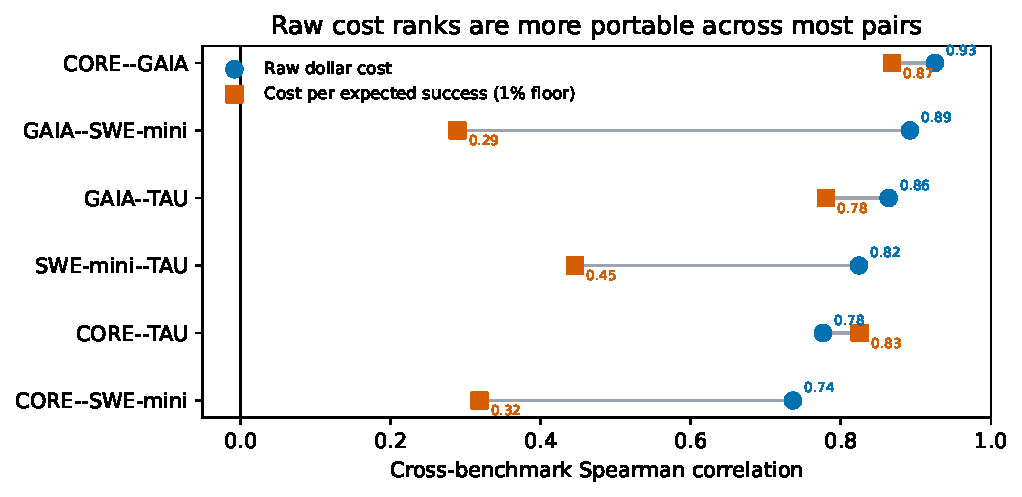
\includegraphics[width=\linewidth]{figures/raw_cost_vs_cost_per_success.pdf}
\caption{Raw-cost versus CPS rank transfer for high-overlap pairs. CPS uses the primary 1\% denominator floor.}
\end{figure}

\subsection{LOBO identifies portable and nonportable raw-cost settings}

In LOLO influence checks, the positive LOBO findings are not single-label artifacts: CORE remains \(\rho\in[0.73,0.91]\), GAIA [0.84,0.92], SWE-mini [0.88,0.92], and TAU [0.79,0.95] across every omission. SciCode is unstable ([-0.50,0.14]); ScienceAgentBench remains negative ([-0.77,-0.43]) but its original \(N=7\) test is non-significant. SciCode's mean accuracy is 2.1\% with 33.3\% zero-accuracy labels; ScienceAgentBench has the narrowest log-cost dispersion. These six-benchmark diagnostics are descriptive and do not identify a domain effect.

\begin{figure}[t]
\centering
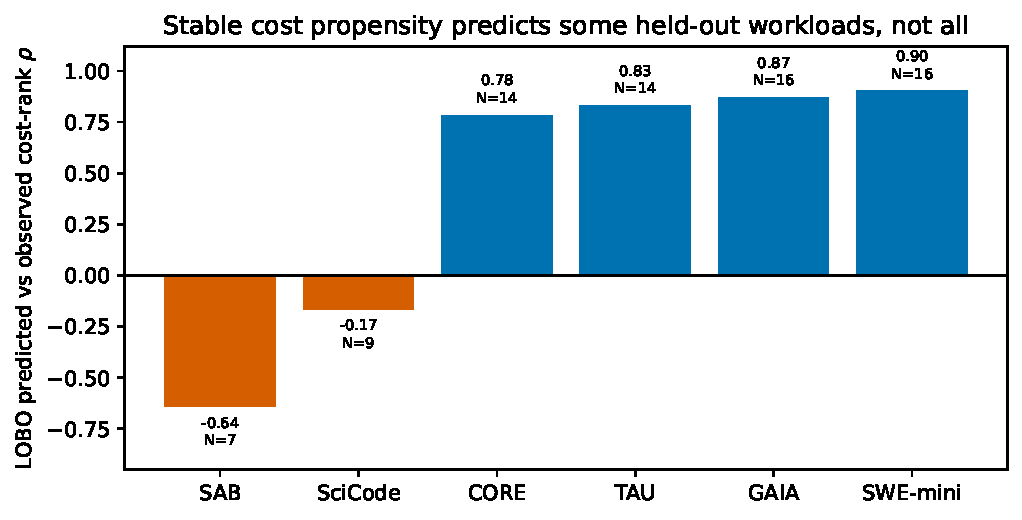
\includegraphics[width=\linewidth]{figures/lobo_cost_portability.pdf}
\caption{LOBO predicted versus observed raw-cost ranks. Blue bars differ from the 20,000-draw label-pairing permutation null at 0.05; orange bars do not.}
\end{figure}

\subsection{Frontier membership is non-universal}

No label tested on at least five workloads appears on every observed accuracy--cost frontier under discrete nondominance, the \hal-inspired hull, or 5\% tolerance. The stronger claim that no label appears on more than 4/6 frontiers is not robust: under tolerance, o4-mini Low appears on 5/6. We therefore retain only the non-universal-winner conclusion.

\section{External matched trajectory study}

\subsection{Data and design}

The \hal{} aggregate CSV cannot identify execution mechanisms because its traces are encrypted. We therefore conduct an external, separate matched trace analysis using public unencrypted Open-SWE-Traces data. We select a documented four-shard boundary sample for MiniMax-M2.5 under OpenHands and SWE-agent. The boundary sample is reproducible but not a random sample of the full corpus. We exact-match task ID and model, exclude duplicate task/model/scaffold records, and obtain 977 pairs.

The trace schema contains resolved status, message roles, explicit tool calls, message text, and reasoning text. It does not contain billed tokens, dollars, provider usage, retries, or latency. We measure trajectory turns, assistant turns, explicit tool calls, tool-result turns, total message characters, and reasoning-message characters. Character counts are tokenizer-free text-volume proxies, not tokens or costs. Paired comparisons use two-sided Wilcoxon signed-rank tests.

\subsection{Scaffold changes trajectory burden at fixed task and model}

OpenHands has lower matched medians: 123 versus 149 trajectory turns, 61 versus 74 assistant turns/tool calls, and 176,708 versus 194,263 total trajectory characters. The OpenHands/SWE-agent median ratio is 0.85 for turns (10,000-bootstrap interval [0.82,0.87]) and 0.85 for tool calls ([0.82,0.86]); OpenHands is lower on 69.7\% of pairs for each. Characters have ratio 0.95 ([0.92,0.98]) and are lower on 55.1\% of pairs. Resolved status has no detected paired difference (\(p=0.197\)). This supports a scaffold difference in observable trajectory structure, not lower tokens, dollar cost, or a causal explanation of \hal{} rankings.

\begin{figure}[t]
\centering
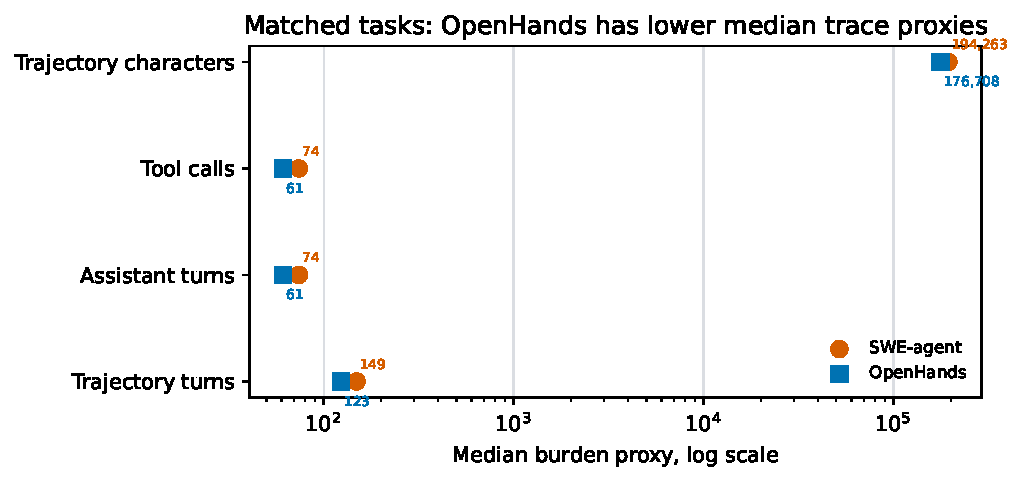
\includegraphics[width=\linewidth]{figures/matched_trace_burden.pdf}
\caption{Matched MiniMax-M2.5 task pairs in the Open-SWE boundary sample (\(N=977\)). Markers show scaffold medians on a log scale for trace proxies, not tokens or dollars.}
\end{figure}

\section{Discussion}

The combined results clarify what a cost-aware agent leaderboard can and cannot establish. Raw dollar-cost rankings are predictive for some held-out workloads, but their portability is largely associated with stable observed displayed-label cost propensity. CPS portability is weaker, so raw cheapness is not interchangeable with deployment efficiency. Independent matched traces further show that scaffolds change measurable execution structure, even when task and model are fixed.

This is a secondary-data analysis with clear construct boundaries. The primary CSV has sparse, nonrandom coverage, mostly single-run rows, and public display labels that omit prompts, tools, budgets, and routing. Cost-propensity adjustment is not provider-price control. CPS is not successful-run cost. The external trace study is not merged with HAL, uses a nonrandom boundary sample, and uses burden proxies rather than billing fields. We cannot compute failure-cost ratios, tail dollar costs, tokens, cache usage, retries, or a true three-dimensional accuracy--cost--reliability frontier from public data. These limitations motivate public release of aggregate usage and outcome telemetry with leaderboard results.

\section{Conclusion}

Observed dollar-cost portability is real in several high-overlap agent benchmark pairs, but it should not be read as a universal deployment-efficiency signal. It is partly persistent label-level cost propensity, weakens after success adjustment, and coexists with substantial scaffold differences in matched trajectory structure. Agent leaderboards should report not only accuracy and raw dollar cost, but also success-adjusted outcomes and trace-level usage fields needed to distinguish price, scaffold, and execution mechanisms.

\bibliographystyle{plainnat}
\bibliography{references}
\end{document}
